% Copyright 2018 Rebecca Skinner
%
% This work is licensed under the Creative Commons
% Attribution-ShareAlike 4.0 International License. To view a copy of
% this license, visit http://creativecommons.org/licenses/by-sa/4.0/
% or send a letter to Creative Commons, PO Box 1866, Mountain View, CA
% 94042, USA.
\documentclass{beamer}

\title{An Introduction to Functional Programming}
\author{Rebecca Skinner}
\date{\today}

\mode<presentation> {\usetheme{metropolis}}

\usepackage[english]{babel}
\usepackage{times}
\usepackage[T1]{fontenc}
\usepackage{hyperref}
\usepackage{listings}
\usepackage{color}
\usepackage{amsmath}
\usepackage{csquotes}
\usepackage{verbatim}
\usepackage{fontspec}
\usepackage{pbox}

\definecolor{comment}{rgb}{145,175,188}
\definecolor{keyword}{rgb}{157,163,199}
\definecolor{string}{rgb}{155,204,174}

\lstset{ % add your own preferences
%  basicstyle=\tiny,
  showspaces=false,
  showtabs=false,
  numbers=none,
  numbersep=5pt,
  showstringspaces=false,
  stringstyle=\color[rgb]{0.16, .47, 0},
  tabsize=1
}

\newcommand{\chref}[3] {
  {\color{#1} \href{#2}{\underline{#3}}}
}

\AtBeginSection[]{
  \begin{frame}
    \vfill
    \centering
    \begin{beamercolorbox}[sep=8pt,center,shadow=true,rounded=true]{title}
      \usebeamerfont{title}\insertsectionnumber \\ \insertsectionhead\par%
    \end{beamercolorbox}
    \vfill
  \end{frame}
}

\AtBeginSubsection[]{
  \begin{frame}
    \vfill
    \centering
    \begin{beamercolorbox}[sep=8pt,center,shadow=true,rounded=true]{title}
      \usebeamerfont{title}\insertsectionnumber.\insertsubsectionnumber\\\insertsubsectionhead\par%
    \end{beamercolorbox}
    \vfill
  \end{frame}
}

\begin{document}
\begin{frame}
  \titlepage{}
  \begin{center}
    \small{\chref{blue}{http://creativecommons.org/licenses/by-sa/4.0/}{LICENSE}}
  \end{center}
\end{frame}

\section{What is Functional Programming?}

\begin{frame}
  \frametitle{Introduction}
  Functional Programming has been growing in popularity, especially
  over the last decade as more languages add first-class support for
  functional programming.

  In this presentation we'll discuss
  \pause
  \begin{itemize}
  \item The history of functional programming
  \item The difference between functional programming and functional languages
  \item Introduce the Haskell programming language
  \end{itemize}
\end{frame}

\begin{frame}
  \frametitle{Alonzo Church and Alan Turing}
  \begin{columns}
    \begin{column}{0.5\textwidth}
      \begin{center}
        \begin{figure}
          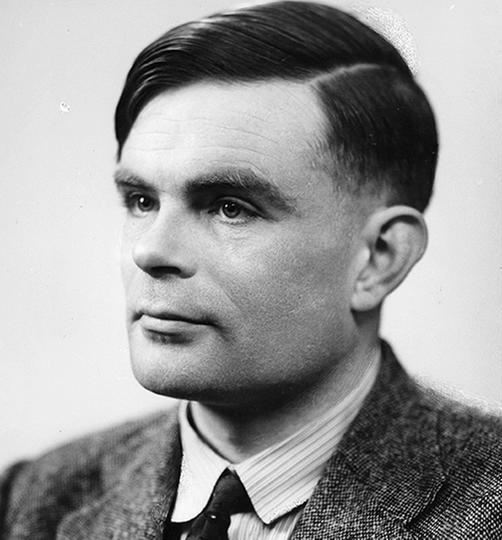
\includegraphics[width=.45\paperwidth]{images/turing.png}
          \caption{Alan Turing}
        \end{figure}
      \end{center}
    \end{column}
    \begin{column}{0.5\textwidth}
      \begin{center}
        \begin{figure}
          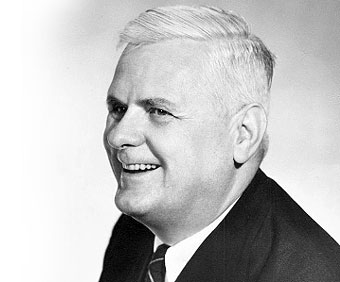
\includegraphics[width=.45\paperwidth]{images/church.jpg}
          \caption{Alonzo Church}
        \end{figure}
      \end{center}
    \end{column}
  \end{columns}
\end{frame}

\begin{frame}
  \frametitle{Timeline of Functional Programming}
  Functional programming has been gaining interest over the last
  decade, but it's roots go back to the very beginnings of the field
  of Computer Science:
  \begin{itemize}
    \item Alonzo Church discovered Lambda Calculus in the 1930's
    \item In 1958 John McCarthy created the first Lisp
    \item In 1968 APL was created, it would go on to influence many
      functional languages
    \item In 1973 ML was created
    \item FP remains interesting mostly to academics for the next 40 years
  \end{itemize}
\end{frame}

\begin{frame}
  \frametitle{Recent Interest in Functional Programming}
  \begin{itemize}
  \item 1998: The release of Half-Life means suddently nerds everywhere recognize the lambda symbol
  \item 2005: Ruby starts to gain popularity, bringing closures, maps, and folds into popularity
  \item 2007: Microsoft introduceds LINQ to .NET 3.5
  \item 2008: Java 8 introduces lambdas, and Java generics start to gain popularity
  \item 2012: The Elm Programming Language is released
  \item 2013: John Carmack mentions Haskell at QuakeCon
  \item 2013: React is released, inciting interest in immutability in the frontend
  \end{itemize}
\end{frame}

\begin{frame}
  \frametitle{History of Functional Programming}
  \begin{center}
    \begin{figure}
      
\includegraphics[height=.70\paperheight]{images/freeman.png}
      \caption{Gordon Freeman: Crowbar and $\lambda$ Calculus Enthusiast}
      \end{figure}
  \end{center}
\end{frame}

\begin{frame}
  \frametitle{Style, Not Languages}
  Functional programming is an approach to software design,
  architecture, and philosophy.  Functional programming isn't about
  the language that you use.
\end{frame}

\begin{frame}
  \frametitle{What Makes Programming Functional?}
  Fundamentally, functional programing is about modeling your program
  using pure mathematical functions- that is functions that always
  return the same output for a given input.  There are a few other
  basics that are needed to do functional programming in any language:
  \begin{itemize}
    \item First class functions
    \item Pure functions
    \item Immutability
    \item Recursion
    \item Strong separation between data structures and values
  \end{itemize}
\end{frame}

\begin{frame}
  \frametitle{Related To Functional Programming}
  Beyond just the core features needed to do FP, there are many
  features that commonly show up in tandem with functional code:
  \begin{itemize}
    \item Pattern Matching
    \item Controlled effects
    \item Flexible type systems
    \item Lazy Evaluation
    \item Currying and Partial Application
  \end{itemize}
\end{frame}

\begin{frame}
  \frametitle{What Makes a Functional Language}
  A functional language is one that facilitates writing programs in a
  functional style.  A pure functional language is one where
  functional programming is the dominant way of writing software in
  the language.
  \begin{columns}
    \begin{column}{0.3\textwidth}
      \begin{itemize}
      \item Haskell
      \item Elm
      \item Idris
      \item Coq
      \item Agda
      \end{itemize}
      Pure Functional Languages
    \end{column}
    \begin{column}{0.3\textwidth}
      \begin{itemize}
      \item Java 8
      \item C++11
      \item Python
      \item Ruby
      \item Javascript
      \end{itemize}
      Functional Languages
    \end{column}
    \begin{column}{0.3\textwidth}
      \begin{itemize}
      \item C
      \item Go
      \item Prolog
      \item SQL
      \item COBOL
      \end{itemize}
      Non-Functional Languages
    \end{column}
  \end{columns}
\end{frame}

\begin{frame}
  \begin{center}
    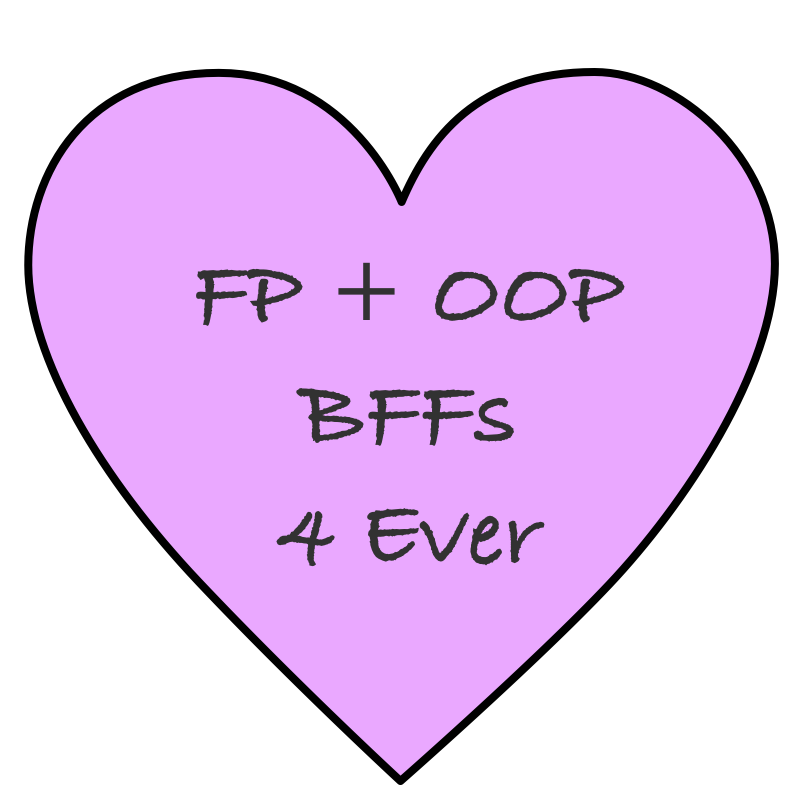
\includegraphics[height=.70\paperheight]{images/bffs.png}
  \end{center}
\end{frame}

\begin{frame}
  \frametitle{FP With Other Paradigms}
  Functional style programming can work well when mixed with other
  programming paradigms like procedural, object oriented, or logic, or
  meta programming.  Mixing FP with OOP is particularly popular, and
  numerous approaches have been developed to mix these two distinctive
  approaches to programming.
\end{frame}

\section{Why Functional Languages Now?}

\begin{frame}
  \frametitle{Modern Interest in an Old Approach}
  After some diminishing interest in functional languages, especially
  lisp, as a means of developing AI in the 1980's there was a drought
  of interest in FP outside of academia.  Commercial and open source
  projects focused on single-dispatch class-based object oriented
  languages like C++ and Java, and on scripting languages like Python
  and Ruby.
\end{frame}

\begin{frame}
  \frametitle{A Surge of Interest}
  In the late 2000's and early 2010's several factors contributed to a
  renewed interest in FP, including:
  \begin{itemize}
  \item 12-factor apps modern cloud architecture
  \item Map-Reduce, Hadoop, and the rise of Big Data
  \item React.js
  \item Scala, Clojure, Elm, and a resurgence in Erlang
  \end{itemize}
\end{frame}

\begin{frame}
  \begin{center}
    
\includegraphics[width=.90\paperwidth]{images/cloud.jpg}
  \end{center}
\end{frame}

\begin{frame}
  \frametitle{FP + Cloud}
  Cloud native applications share many of the same concerns as
  traditional functional programs.  Whether it's understanding how to
  scale and orchestrate processes like Erlang and Exliser, or
  threading state through a series of stateless data transformations,
  the techniques pioneered by functional programming can be of great
  benefit when building cloud applications.
\end{frame}

\section{Introducing Haskell}

\begin{frame}
  \frametitle{A Joke About Burritos}
  \begin{center}
    
\includegraphics[width=.80\paperwidth]{images/haskell.png}
  \end{center}
\end{frame}

\begin{frame}
  \frametitle{A Bit About Haskell}
  Haskell is a pure functional programming language.  It's one of the
  more well known members of the ML family, and is perhaps the most
  widely used pure functional language in industry.
\end{frame}

\begin{frame}
  \frametitle{Some Facts About Haskell}
  \begin{itemize}
  \item Used at: Rackspace, Facebook, Microsoft, Target, Starbucks, and many others.
  \item Over 10,000 packages available on Hackage
  \item Runtime speed and memory footprint are on the order of efficient languages such as C, C++, and Java.
  \item Typically compiled to native code or LLVM bytecode.
  \item Easy interoperability with C and C++
  \end{itemize}
\end{frame}

\begin{frame}
  \frametitle{Some Other Facts About Haskell}
  \begin{itemize}
    \item Of the 10,000 packages on Hackage, some 8,000 of them are probably remnants of someone's PhD Thesis
    \item For every 5 haskell programs written, 6 monad tutorials are posted on someone's blog
    \item Readability is often considered somewhere between ``obfuscated perl'' and ``c'thulu''
    \item {\tt return} in haskell is the most poorly chosen function name in the history of programming languages
  \end{itemize}
\end{frame}

\begin{frame}
  \begin{center}
    \begin{figure}
      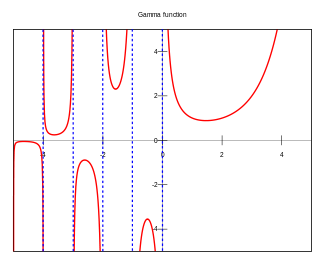
\includegraphics[height=.70\paperheight]{images/gamma.png}
      \caption{Haskell's Learning Curve, Visualized}
    \end{figure}
  \end{center}
\end{frame}

\subsection{Some Examples of Haskell}

\begin{frame}[fragile]
  \frametitle{Hello World}
\begin{lstlisting}[language=haskell]
module Main where
main = print "hello, world"
\end{lstlisting}
\end{frame}

\begin{frame}[fragile]
  \frametitle{quicksort}
\begin{lstlisting}[language=haskell]
module Quicksort where
quicksort [] = []
quicksort (p:xs) =
  (quicksort lesser) ++ [p] ++ (quicksort greater)
  where
    lesser = filter (< p) xs
    greater = filter (>= p) xs
\end{lstlisting}
\end{frame}

\begin{frame}[fragile]
\begin{lstlisting}[language=haskell]
module Echo where
import System.IO
import Control.Monad
echo = do
  toEcho <- getLine
  unless (null toEcho) $ do
    putStrLn toEcho
    echo
main = do
  putStrLn "Echo some words! (empty line to quit)"
  echo
\end{lstlisting}
\end{frame}

\begin{frame}
  \frametitle{Getting Started with Haskell}
  Here are some handy pointers to get you started learning more abut
  haskell:
  \begin{itemize}
    \item \href{http://haskellbook.com}{Haskell from First Principals}
    \item \href{https://en.wikibooks.org/wiki/Haskell}{Haskell Wikibook}
    \item \href{http://haskellstack.org}{The Stack Tool}
    \item \href{https://atom.io/packages/ide-haskell}{Haskell IDE (atom)}
    \item \href{https://commercialhaskell.github.io/intero/}{Haskell IDE (emacs)}
  \item \href{http://dev.stephendiehl.com/hask/}{What I Wish I Knew When Learning Haskell}
  \end{itemize}
\end{frame}
\section{Questions?}

\end{document}
